\documentclass[SoftwareDesign/SoftwareDesign_main.tex]{subfiles}

\begin{document}
\section{Design af Login}
I dette afsnit præsenteres designet af den, hvor en bruger, der ønsker at logge på sin konto på applikationen. Dette afsnit beskriver designet af vores view og den udseende på siden, samt design af funktionaliteten.

\subsection{Design af View til Login}

\begin{figure}[H]
    \centering
    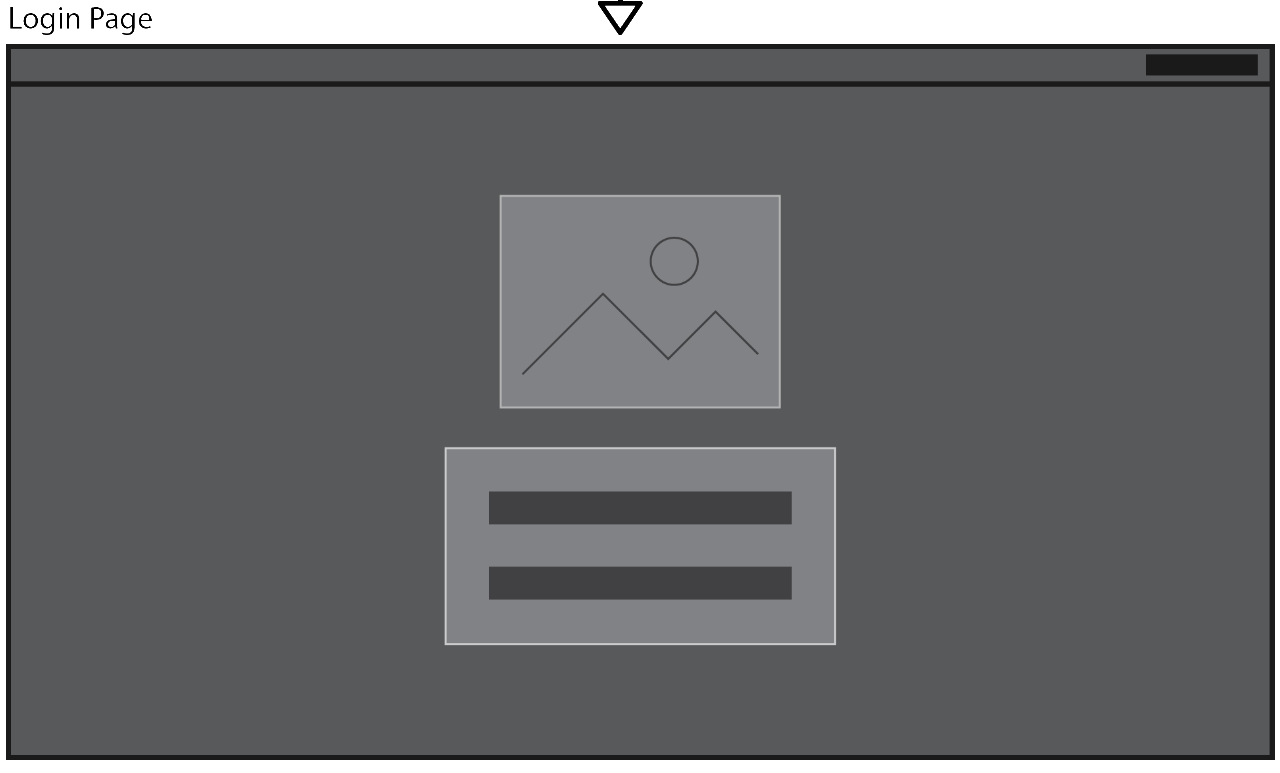
\includegraphics[width=\textwidth]{SoftwareDesign/MVVMDesigns/Graphics/LoginWireframe.png}
    \caption{Wireframe af login}
    \label{fig:LoginWireframe}
\end{figure}

Ud fra Wireframet i figur \ref{fig:LoginWireframe} kan der ses layout af siden. Det overordnede wireframe viser funktionalitet angående navigation, mellem siderne. Loginsiden skal kun navigere til startsiden og til loginsiden. Siden skal navigere videre til startpage, hvis brugeren logger in med oprettet konto. Brugeren bliver navigeret til Usersignup page, hvis brugeren ikke har oprettet en konto og derved skal lave en. 


\subsection{Design af Viewmodel til Login}
Når en bruger prøver at logge in på sin konto, skal brugerens information overholde nogen regler, som f.eks at der skal være et x antal langt kodeord, før det kan godkendes til at være en gyldig kodeord. Der lavet et antal validering af brugerens kodeord og email, som kan udskrive til brugeren, hvilken af brugerens information ikke godekendes. Da koden fra brugeren er forutroligt information skal det ikke kunne ses i applikationen, som løsning bliver der benyttet securestring til koden, yderlig information af hvordan det fungerer kan ses på UserSignUp. ------- Mangler REF ----------. Der bliver navigeret videre hen til Start page og Usersignup page via delegate commands.    




\end{document}